\documentclass[12pt,a4paper]{article}

\usepackage[left=3cm, right=3cm, top=2.5cm, bottom=2.5cm]{geometry}
\usepackage{setspace}
\usepackage{amsmath}
\usepackage{tikz}
\usepackage{pgfplotstable}
\usepackage{titlesec}
\usepackage{bm}
\usepackage{tcolorbox}
\tcbuselibrary{skins}
\usepackage{empheq}
\usepackage{booktabs}
\usepackage{caption}
\usepackage{hyperref}
\usepackage{fancyhdr}
\hypersetup{
    colorlinks=true,
    linkcolor=black,
    filecolor=magenta,      
    urlcolor=cyan,
    pdfpagemode=FullScreen,
    }
\usepackage{graphicx}
\graphicspath{ {./images/} }


\titleformat{\section}{\Large\bfseries}{\thesection}{1em}{}
\titleformat{\subsection}{\large\bfseries}{\thesubsection}{1em}{}


\renewcommand{\contentsname}{Table des Matières}
%\renewcommand{\baselinestretch}{1.5}

\title{Étude du Pendule Simple : Analyse des Oscillations Harmoniques}
\author{Liviu Arsenescu, Cătălin Bozan}
\date{05.03.2024}

\newtcbox{\mymath}[1][]{%
    nobeforeafter,
    math upper,
    tcbox raise base,
    enhanced,
    colframe=black,
    colback=white,
    boxrule=1pt,
    drop shadow={
        shadow xshift=3pt,
        shadow yshift=-3pt,
        opacity=1
    },
    #1
}

\pagestyle{fancy}
\fancyhf{}
\rhead{
\includegraphics[width=4cm]{hearclogo.png}}
\lhead{\thepage}
\setlength{\headsep}{30pt}

\begin{document}
    \pagenumbering{gobble}
    \begin{titlepage}
        \begin{center}
            \vspace*{\fill}
            \Huge \textbf{Étude du Pendule Simple :} \\
            \Huge \textbf{Analyse des Oscillations Harmoniques} \\
            \Large Rapport du Laboratoire \\
            \begin{figure}[h]
                \centering
                
\includegraphics[width=7cm]{hearclogo.png}
            \end{figure}
            \vspace{\fill}
            \Large Liviu Arsenescu, Cătălin Bozan \\
            05.03.2024

            \vspace*{\fill}
        \end{center}
    \end{titlepage}

    \thispagestyle{empty}
    \tableofcontents
    \newpage

    \pagenumbering{arabic}
    \section{Objectifs du laboratoire}
    \begin{itemize}
        \item Démontrer expérimentalement le fait que la période ne dépend pas de la masse
        \item Vérifier la formule de la période d'un pendule
        \item Trouver l'accélération gravitationnelle de la terre
    \end{itemize}

    \section{Éléments théoriques}
    \subsection{Les différentes quantités rencontrées}
    \begin{itemize}
        \item $\bm{\theta}$ - l'angle entre la verticale et le pendule
        \item \textbf{L} - la longueur du fil
        \item \textbf{T} - la période du pendule
        \item \textbf{m} - masse d'objet
        \item \textbf{s} - la position de la masse
        \item \textbf{g} - l'accélération gravitationnelle de la terre
    \end{itemize}
    \subsection{La formule fondamentale du pendule}
    La position de la masse suspendue est calculée à l'aide de la formule suivante: 
    \begin{equation*}
        s=L\theta,
    \end{equation*}
    La deuxième loi de Newton ($\sum_{i=1}^{n} F_i=ma$) selon l'axe tangentiele s'écrit:
    \begin{equation*}
        -mgsin(\theta) = m\frac{d^2s}{dt^2}
    \end{equation*}
    où $-mgsin(\theta)$ est l'équation obtenue pour la seule force agissant sur l'objet (P - poids), et $\frac{d^2s}{dt^2}$ est l'accélération totale du système, obtenue en dérivant deux fois la position. \\
    On sait que $\frac{d^2s}{dt^2} = L\frac{d^2\theta}{dt^2}$ (L - constante). Alors:
    \begin{align*}
        -mgsin(\theta)&=mL\frac{d^2\theta}{dt^2} \\
        -\frac{g}{L}sin(\theta)&=\frac{d^2\theta}{dt^2} \\
        \frac{d^2\theta}{dt^2}+\frac{g}{L}sin(\theta)&=0
    \end{align*}
    Pour notre expérience, nous n'utilisons que de petits angles, ce qui nous permet de faire l'approximation suivante: $sin(\theta) \approx \theta$. Le pendule simple devient alors un système oscillatoire harmonique, décrit par l'équation suivante:
    \begin{empheq}[box={\mymath}]{equation*}
        \frac{d^2\theta}{dt^2}+\frac{g}{L}\theta=0
    \end{empheq}
    En comparant cette équation avec l'équation du mouvement oscillatoire harmonique ($\frac{d^2x}{dt^2}+\omega^2x(t)=0$), nous obtenons:
    \begin{center}
        \vspace{-\baselineskip}
        \begin{minipage}{0.2\linewidth}
            \begin{empheq}[box={\mymath}]{equation*}
                \omega=\sqrt{\frac{g}{L}}
            \end{equation*}
        \end{minipage}%
        \begin{minipage}{0.1\linewidth}
            \begin{center}
                et
            \end{center}
        \end{minipage}%
        \begin{minipage}{0.2\linewidth}
            \begin{empheq}[box={\mymath}]{equation*}
                T=\frac{2\pi}{\omega}=2\pi\sqrt{\frac{L}{g}}
            \end{equation*}
        \end{minipage}
    \end{center}
    Cette approche mathématique permet de tirer les conclusions suivantes:
    \begin{itemize}
        \item La période ne dépends pas de la masse de l'objet
        \item La période est proportionnelle à la racine carrée de la longueur
        \item Nous pouvons estimer expérimentalement la norme d'accélération gravitationnelle à l'aide de la formule: 
        \begin{equation*}
            g=\frac{4\pi^2L}{T^2}
        \end{equation*}
    \end{itemize}

    \section{Manipulation}
    \subsection{Matériel}
    \begin{minipage}{0.5\textwidth}
        \begin{itemize}
            \item Socle
            \item Tiges
            \item Noix-double
            \item Tige-pince
            \item Diverses masses
        \end{itemize}
    \end{minipage}
    \begin{minipage}{0.5\textwidth}
        \begin{itemize}
            \item Fil non élastique
            \item Ruban métrique
            \item Camera vidéo
            \item Ordinateur
        \end{itemize}
    \end{minipage}
    \subsection{Configuration}
    La tige est fixée verticalement au socle. En utilisant la noix-double, on fixe horizontalement un'autre tige qui dispose d'un pince à l'extrémité. On a fait une boucle à l'extrémité de la ficelle et l'avons utilisée pour suspendre le poids.
    Ensuite, on a utilisé la pince pour saisir la corde, ce qui nous permet de modifier la longueur du pendule. Une balance a été utilisée pour peser les poids. \\
    Un téléphone portable équipé d'une caméra capable d'enregistrer 60 images par seconde et le programme de montage vidéo \href{https://kdenlive.org}{Kdenlive} ont été utilisés pour enregistrer et chronométrer la période du pendule. \\

    \begin{figure}[h]
        \centering
        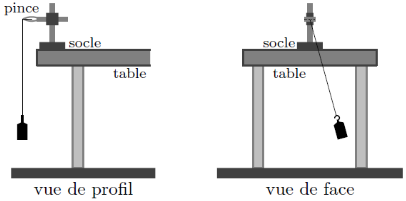
\includegraphics[width=7cm]{laboPhysiqueBPendule.png}
    \end{figure}

    \section{Mesures}
    \subsection{Manière de mesurer}
    Pour reduire l'incertitude, on n'a pas utilisé de chronomètre pour mesurer le temps, mais on a pris une vidéo avec une caméra de 60 cadres par seconde. Ensuite, on a analysé la vidéo à l'aide d'un logiciel de montage, pour mieux voir les cadres du début et de la fin. \\
    Bien que les instructions du laboratoire indiquent que nous devrions enregistrer 10 périodes, pendant le laboratoire on a eu une erreur avec les vidéos, ce qui nous a permis d'enregistrer seulement 7 périodes. Cela n'a pas eu un grand impact sur l'incertitude. \\
    Pour le reste des mesures(longueur, masse), on a suivi les instructions de laboratoire.
    \section{Analyse des mesures et résultats}
    \subsection{Période d'oscillation \textit{T} en fonction de la masse \textit{m}}
    Pour cette expérience, on a une longueur fixe pour le fil et on a augmenté la masse. \\
    Les valeurs suivantes restent constantes pour chaque mesure:
    \begin{itemize}
        \item Longueur: $L=80.0cm$
        \item Incertitude de la longueur: $\Delta L=\pm 0.4cm$
        \item Incertitude de la masse: $\Delta m=\pm 0.01g$
        \item Incertitude de 7 périodes: $\Delta 7T=\pm 0.05s \Rightarrow \Delta T=\pm 0.008s$
    \end{itemize}
    Le reste des valeurs peut être représenté dans un tableau:
    \begin{table}[htbp]
        \centering
        \begin{minipage}{0.4\textwidth}
            \begin{tabular}{c|c|c|c}
                \textbf{No.} & \textbf{m(g)} & \textbf{7T(s)} & \textbf{T(s)} \\
                \toprule
                1 & 19.96 & 12.52 & 1.788 \\
                2 & 49.76 & 12.60 & 1.800 \\
                3 & 99.63 & 12.55 & 1.792 \\
                4 & 199.69 & 12.57 & 1.795 \\
                5 & 499.46 & 12.52 & 1.788 \\
            \end{tabular}
        \end{minipage}%
        \begin{minipage}{0.6\textwidth}
            \centering
            \fbox{%
                \begin{tabular}{rcl}
                    Symb. & & description \\
                    \toprule
                    m(g) & - & masse en grammes \\
                    7T(s) & - & mesure de 7 périodes en secondes \\
                    T(s) & - & période en secondes \\
                \end{tabular}%
            }
        \end{minipage}
    \end{table} \\
    On peut utiliser cet ensemble de données pour faire un graphique: \\
    \pgfplotstableread[col sep=comma]{plotData/plotExpI.csv}\expIdata
    \begin{tikzpicture}[scale=1]
        % Scatter plot
        \begin{axis}[
            xlabel={$m$},
            ylabel={$T$},
            legend pos=north east,
            legend style={at={(0.7,0.75)}, anchor=south},
            grid=both,
            width=1\textwidth,
            height=0.3\textheight,
            x tick label style={
                /pgf/number format/.cd,
                precision=2,
                fixed,
                fixed zerofill,
            },
            y tick label style={
                /pgf/number format/.cd,
                precision=3,
                fixed,
                fixed zerofill,
            },
            xmin=15,
            xmax=515,
            ymin=1.76,
            ymax=1.82,
        ]
            \addplot+[only marks, mark=x, error bars/.cd, x dir=both, x explicit, y dir=both, y explicit] table[x=m, x error=err_m, y=T, y error=err_T] {\expIdata};

            % Linear regression line
            \addplot [red, thick] table[
                y={create col/linear regression={y=T}}
            ] {\expIdata};
            \xdef\slope{\pgfplotstableregressiona}
            \xdef\intercept{\pgfplotstableregressionb}

            % Add the equation of the line
            \addlegendentry{Données}
            \addlegendentry{Régr. Lin.: $y = \pgfmathprintnumber{\slope}x + \pgfmathprintnumber{\intercept}$}
        \end{axis}
    \end{tikzpicture}
    Après l'analyse du graphique, on constate que la pente est en fait incroyablement faible, et qu'elle tend vers 0 ($-1.06\cdot10^{-5}$). \\
    On sait qu'un graphique dont la pente est égale à 0 nous donne une valeur constante de la fonction sur laquelle on travaille. \\
    Avec le fait que nos mesures étant très proches des prédictions théoriques, on peut conclure que la période du pendule ne dépend pas de la masse de l'objet.
    \subsection{Période d'oscillation \textit{T} en fonction de la longueur \textit{L}}
    Pour cette expérience, on a la masse qui reste fixe, et on a augmenté la longueur du fil. \\
    Les valeurs suivantes restent constantes pour chaque mesure:
    \begin{itemize}
        \item Masse: $m=199.42g$
        \item Incertitude de la masse: $\Delta m=\pm0.01g$
        \item Incertitude de 7 périodes: $\Delta 7T=\pm0.05s\Rightarrow \Delta T=\pm0.008s$
    \end{itemize}
    Le reste des valeurs peut être représenté dans un tableau:
    \begin{table}[htbp]
        \centering
        \begin{minipage}{0.55\textwidth}
            \begin{tabular}{c|c|c|c|c}
                \textbf{No.} & \textbf{L(cm)} & \textbf{$\bm{\Delta}$L(cm)} & \textbf{7T(s)} & \textbf{T(s)} \\
                \toprule
                1 & 10 & 3 & 4.48 & 0.640 \\
                2 & 20 & 3 & 6.20 & 0.885 \\
                3 & 30 & 3 & 7.68 & 1.097 \\
                4 & 40 & 4 & 8.85 & 1.264 \\
                5 & 50 & 4 & 9.93 & 1.418 \\
                6 & 60 & 4 & 10.83 & 1.547 \\
                7 & 70 & 4 & 11.77 & 1.681 \\
                8 & 80 & 5 & 12.55 & 1.792 \\
                9 & 90 & 5 & 13.31 & 1.901 \\
                10 & 90.5 & 5 & 14.05 & 2.007 \\
            \end{tabular}
        \end{minipage}%
        \begin{minipage}{0.45\textwidth}
            \centering
            \fbox{%
                \begin{tabular}{rcl}
                    Symb. & & description \\
                    \toprule
                    L(cm) & - & longueur en centimetres \\
                    $\Delta$L(cm) & - & incertitude de la longueur \\
                    7T(s) & - & 7 périodes en secondes \\
                    T(s) & - & période en secondes \\
                \end{tabular}%
            }
        \end{minipage}
    \end{table} \\
    \section{Synthèse et conclusion}
    Suite aux deux expériences et aux mesures effectuées, on constate que, comme le dit la théorie, la période du pendule varie en fonction de la longueur de la corde, et qu'elle est indépendante du poids. \\
    En outre, nous avons réussi à déduire la constante d'accélération gravitationnelle qui est très proche de la constante réelle $\approx 9.81$.
\end{document}

